\documentclass[a4paper, 12pt]{article}
\usepackage{comment} 
\usepackage{fullpage}
\usepackage[hidelinks]{hyperref}
\usepackage{amsmath}
\usepackage{environ}
\usepackage{graphicx}
\usepackage{tabto,enumitem}

\begin{document}
\noindent
\large\textbf{SOEN 6011 SEP} \hfill \textbf{Mahavir Patel} \\
\normalsize Problem 1 \hfill \textbf{40198619} \\
Function 6 :  $B(x,y)$ Beta Function \hfill Date: 05/07/2022 \\

\section{Introduction}
The beta function is a special function that belongs to the first category of Euler's integrals. The beta function is denoted by the symbol  "${B}$". $B(x,y)$ refers to the beta function, where $x$ and $y$ are real-valued parameters. \\
The formula of \textbf{$B(x,y)$} is\footnote{\href{https://en.wikipedia.org/wiki/Beta\_function}{https://en.wikipedia.org/wiki/Beta\_function}}:
    \begin{itemize}
        \item $B(x,y) = \frac{(x-1)! (y-1)!}{(x+y-1)!}$ \text{For positive integers}
        \item $B(x,y)$ = $\int_{0}^{1} {t^{x-1}}{(1-t)^{y-1}} dt$ \text{For positive real numbers}
    \end{itemize}

\section{Properties of Beta Function}
    \begin{itemize}[noitemsep]
        \item Beta function is symmetric which means its beta value is independent of the order of its parameters: $B(x,y) = B(y,x)$
        \item $B(x,y) = B(x,y+1) + B(x+1,y)$
        \item $B(x,y+1) = B(x,y) \cdot [\frac{y}{x+y}]$
        \item $B(x+1,y) = B(x,y) \cdot [\frac{x}{x+y}]$
        \item $B(x,y) . B(x+y,1-y) = \frac{\pi}{x}\sin{\pi y}$
        \item Beta function in terms of Gamma functions as:
            $B(x,y)=\frac{\Gamma x \Gamma y}{\Gamma (x+y)}$ , When x and y are positive whole number then it follows the form of gamma function.
        \item The beta function can be extended to a function with more than two arguments:\\ $B(X_{1},X_{2},...X_{n}) = \frac{\Gamma X_{1} \Gamma X_{2} ... \Gamma X_{n}}{ \Gamma (X_{1} + X_{2} + ... + X_{n})}$
    \end{itemize}

\section{Domain and Co-Domain}
The domains of real numbers are where the beta function is defined. The limitations of the integral function determine the beta function's co-domain. the beta function is defined For real values that are positive and greater than zero. nonetheless, there are other ways to write a beta function, for example, \\
    \begin{itemize}
        \item $B(x,y)$ = $\int_{0}^{\frac{\pi}{2}} (\sin \theta)^{2x-1} (\cos \theta)^{2x-1}$ where $x>0$ and $y>0$
        \item $B(x,y)$ = $\int_{0}^{\infty} \frac{t^{x-1}}{(1+t)^{x+y}} dt$  where $x>0$ and $y>0$
    \end{itemize}
for the variables domain is (0,${\infty}$] and based on the beta function's integral limits co-domain can be defined.\\

\newpage
\section*{Context of Use Model}

\begin{figure}[h]
    \centering
    \begin{center}
    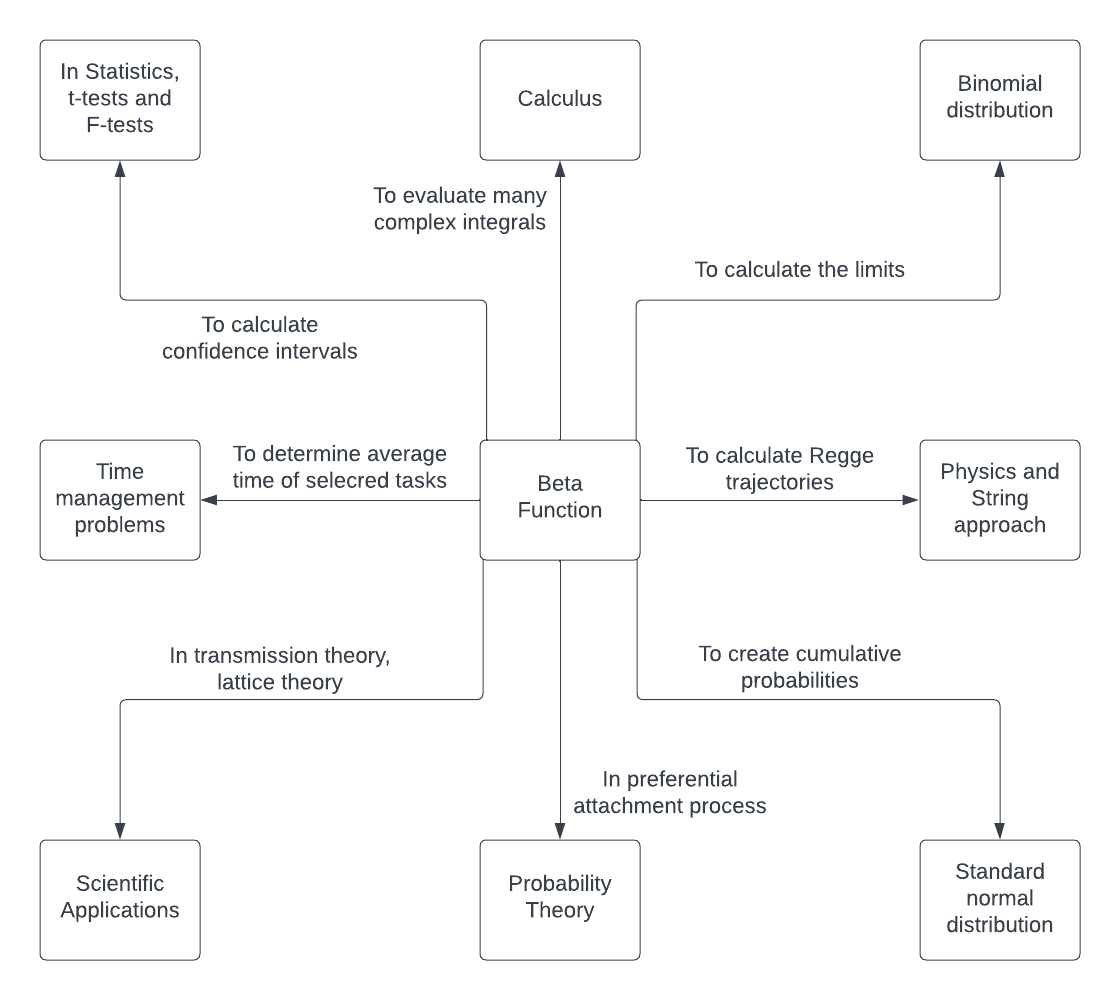
\includegraphics[width=1.0\linewidth]{Images/beta_contextmodel.png}    
    \end{center}
    \caption{Context of use model.}
    \label{fig:Context of Use Model.}
\end{figure}

\end{document}
